%% Single column version for a Springer Nature journal (Scientific Reports style).
%% This file is the text source. srep/make_srep_docx.py turns it into the Word file.
%% Lines like %%TABLE eaai:tab:ablation%% pull the table of that label from eaai/manuscript.tex,
%% and %%GENTABLE name%% inserts a table generated from the result files, so no number is typed twice.

\title{Detecting Prediction Collapse Caused by Pooled Feature Normalization in Space-Trajectory Screening}

\begin{abstract}
Monte Carlo trajectory campaigns spend much of their computing time on runs that are already sure to fail, and machine learning screens that stop such runs early are an attractive way to save that time. These screens depend on routine preprocessing choices. We show that one common choice, fitting a single feature scaler to data pooled across target groups with very different scales, can make a Transformer screen give almost the same prediction for every mission of a target. On Venus the spread of the predictions falls to 3.11e-05 and the AUC falls from 0.9999 to 0.6037, while an XGBoost baseline on the same arrays stays near perfect and a pooled validation score shows the damage only in part. Across five seeds the collapse occurs on four. We propose a simple check, the spread of the predictions within each group, which needs no labels at run time. With a threshold set on validation runs it flags the four collapsed runs out of 60 and no working run, and it raises no alarm on a second dataset of turbofan engines. The work is relevant to any learned screen trained on grouped data.
\end{abstract}

\begin{keywords}
feature normalization; prediction collapse; model diagnostics; deep learning; Monte Carlo simulation; trajectory screening
\end{keywords}

\section{Introduction}
\label{sec:intro}

Designing a space mission is not done with a single trajectory. Engineers run large Monte Carlo campaigns, in which thousands of trajectories are simulated with small random changes to the launch and the engine burns, to see how often the mission still reaches its target. NASA's TESS mission, for example, used a large dispersion campaign of this kind to set its trajectory design \cite{nickel2016}. Every one of these trajectories has to be propagated, which means that a numerical integrator follows the spacecraft forward in time under the gravity of the Sun and the planets. For transfers to the outer planets one run covers years of simulated flight, so a campaign is expensive.

A large share of that cost is wasted. In our campaigns most of the compute is used on runs that were already sure to fail when they left the parking orbit. One line of work makes each propagation cheaper \cite{massari2017,jia2022}. Another replaces part of an expensive simulation with a learned surrogate \cite{yin2022}. A third, simpler idea is to watch the first part of each trajectory and stop the runs that are going to fail. We call such a model a screen. Machine learning is a natural fit for it, and learned models are already used widely in astrodynamics \cite{izzo2019survey,izzo2024}.

A learned screen is more than a network. It is a pipeline, and one of its quiet steps is feature scaling. Before the data reach the network, every feature is shifted and divided by a typical size, so that features measured in very different units become comparable. This step is old and well understood \cite{sola1997,huang2023}, and it is usually done with one line of code. In our data, however, the features come from seven different target planets, and their ranges differ by orders of magnitude. If one scaler is fitted to all targets of a group together, the large differences between targets set the scale, and the small differences between missions of the same target, which are the ones that decide success or failure, are squeezed close to zero.

This is what happened in our screen. The model ended up giving a single, almost constant probability of failure to every mission of a target. That a pooled scaler can do this is not surprising. The difficulty is that it is easy to miss. A pooled validation score shows the damage only in part: in the controlled ablation of Section~\ref{sec:results}, the AUC over the three targets of a group falls from 0.9995 to 0.875, while the AUC of the failed target alone is 0.687. A gradient boosted tree trained on the same scaled arrays, which is the usual sanity check, scores almost perfectly, because trees split on the order of the values and the rescaling does not change that order. Both checks can leave the engineer with the impression that the data are fine and that only the network needs tuning.

The failure can be described as a preprocessing error, and its remedy, scaling each group separately, is simple. The contribution of this paper is not the remedy. It is a careful description of a failure that a pooled validation score shows only in part and that the tested scale-invariant baseline does not show, together with a check on the spread of the predictions that does show it. The problem is not specific to astrodynamics. Any learned model trained on grouped data, such as engines running under different operating conditions or sensors at different sites, can meet the same failure.

The main contributions of this work are as follows.

\begin{itemize}
\item A controlled decomposition of the collapse. Keeping the model, the data split and the training fixed, we change only how the scaling statistics are pooled, and show that pooling over time within one target is harmless, while pooling across targets can make the model output a constant.
\item An analysis of why the usual checks miss it. A tree baseline on the same input is not affected by this kind of rescaling, and a pooled validation score averages the failed target with the healthy ones.
\item A simple diagnostic, the spread of the predictions within each group, with a fully stated evaluation protocol, a sensitivity analysis, a comparison with other summaries of the predictions, statistical tests, and checks on batch size and calibration.
\item A second, public dataset (NASA turbofan engines) on which the same pooling shrinks the signal without breaking the model, and an economic analysis that places the learned screen in its operational context.
\end{itemize}

The rest of the paper is organized as follows. Section~\ref{sec:review} reviews related work on machine learning in astrodynamics, on feature normalization, and on checks for degenerate models. Section~\ref{sec:method} describes the simulated data, the scaling settings, the models, the diagnostic and the statistical methods. Section~\ref{sec:results} reports the experiments. Section~\ref{sec:discussion} discusses what the results mean for mission assurance and what they do not show. Section~\ref{sec:conclusion} concludes the paper.

\section{Literature review}
\label{sec:review}

\subsection{Machine learning in astrodynamics and simulation screening}

Neural networks have been applied successfully in astrodynamics for trajectory optimization and for approximating optimal control \cite{izzo2019survey,izzo2024,sanchez2018}, for estimating the cost of a transfer without a complete propagation \cite{li2020deep,izzo2019ml}, and for learning robust low-thrust guidance policies that are then certified through Monte Carlo campaigns \cite{zavoli2021}. Learned models are also used to improve orbit predictions from publicly available tracking data \cite{peng2019}, and reduced models make the propagation of orbit uncertainty cheaper than plain sampling \cite{balducci2017}.

Spacecraft telemetry is another large area. Learned models detect anomalies and faults in telemetry streams \cite{naik2020}, including attention-based models of the same family as ours \cite{jiang2023}, and careful pipelines based on recurrent networks perform well when every channel is processed correctly \cite{hundman2018}. Recent work also shows how easily the reported performance of such detectors is overestimated, and that simpler methods can match complex ones once the evaluation is done carefully \cite{herrmann2024}. A public benchmark for anomaly detection in satellite telemetry is now available \cite{kotowski2024}.

Screening itself, where a learned model decides which of a very large number of candidate cases get a full analysis, is already established. An ESA competition used real conjunction data to rank collision risks \cite{uriot2020,acciarini2021}, and a benchmark compared deep approaches with the classical filters they would replace in conjunction screening \cite{stevenson2023}. The last one is the closest setting to ours: a screening task on a deterministic astrodynamics simulator, measured against non-deep baselines. We could not find an article that considers early termination of individual Monte Carlo trajectory runs, as we do in Section~\ref{sec:screen}. The closest work makes each propagation cheaper rather than deciding which propagations to start \cite{massari2017,jia2022}, or uses learned surrogates in place of parts of a simulation \cite{yin2022}.

\subsection{Feature normalization in deep learning and time series}

Normalization is central to training deep networks, and there are standard layers for it (batch, layer, group and instance normalization) \cite{ioffe2015,ba2016,wu2018,ulyanov2016,huang2023}. It has long been known that the ability of a network to train, and not only the speed at which it trains, depends on how the inputs are scaled \cite{sola1997}. These layers also make assumptions about their input. They assume that the feature statistics are stationary, or that they are comparable within each pooling axis. When data from several sources with very different ranges are measured with the same scaler, that assumption is broken before the first layer runs.

Normalization has also been studied for time series on its own. ST-Norm splits it into a temporal part and a spatial part for forecasting models \cite{deng2021}, and Deep Adaptive Input Normalization learns the scaling from the data \cite{passalis2020}. Those papers aim at a more accurate model. We ask a different question: how can a poor scaling choice break a model without anyone noticing? What we add is a controlled decomposition showing that pooling in general does not do the damage, only pooling across groups, and the observation that the resulting model is not a weak model but a constant one.

\subsection{Shortcut learning, degenerate models and checks on machine learning pipelines}

When a shortcut is available, a network easily learns the easy signal and takes the shortcut instead of the intended structure \cite{geirhos2020,shah2020}. Work on Clever Hans behavior shows that models can score well for reasons that have nothing to do with the task \cite{lapuschkin2019}. When groups have very different scales, there is a particularly clean shortcut: the distance between the group centers. A model of this type can learn the difference between groups, and can reach a high AUC on a mixed validation set while performing no better inside the individual groups. The failure is also not a modeling problem but a pipeline problem, of the kind that lives in shared preprocessing code that no single model owns \cite{chaudhary2018}.

Tree ensembles perform well on tabular and physical data, often matching or beating deep models \cite{chen2016,grinsztajn2022,shwartz2022,ke2017,pasaribu2024}, and many practitioners use a tree as a baseline for that reason. Their splits are axis aligned and based on thresholds, so a monotone rescaling of a feature keeps the available ordering. That useful invariance is exactly why the tested XGBoost baseline misses this particular failure when it receives the same transformed arrays. It does not mean that tree baselines are unable to find preprocessing errors in general.

The word collapse also needs care. Neural collapse describes the geometry of the internal representations and the classifier in the final phase of training, after the training error vanishes \cite{papyan2020}. Our outcome is different: the predictions for distinct missions become nearly constant after cross-group scaling. Work on predictive uncertainty under shift shows that confidence and calibration can get worse when the deployment data change \cite{ovadia2019}, and two-sample tests can detect a change between reference and incoming feature distributions without target labels \cite{rabanser2019}. Rubrics for production readiness call for monitors on data, models and serving pipelines rather than a single held-out score \cite{breck2017}. Table~\ref{tab:related-comparison} sets out how these approaches relate to ours.

%%TABLE eaai:tab:related-comparison%%

\subsection{Research gap}

Taken together, the literature offers ways to normalize data well, ways to detect shortcuts and shift, and general advice to monitor pipelines. It does not describe what happens when one scaler is shared across groups of a sequential dataset, why the standard tree baseline cannot see the resulting failure, or how to detect it cheaply. It also does not study learned screens that stop individual Monte Carlo trajectory runs early. This paper addresses those gaps.

\section{Methodology}
\label{sec:method}

\subsection{Overview}

Figure~\ref{fig:pipeline} summarizes the study. A trajectory simulator produces the missions. A short window of telemetry from the start of each flight is scaled in one of three ways and passed to two models: a Transformer screen and an XGBoost baseline. Three checks are then compared: a pooled AUC over a group of targets, the baseline on the same input, and the spread of the predictions within each target.

\begin{figure}
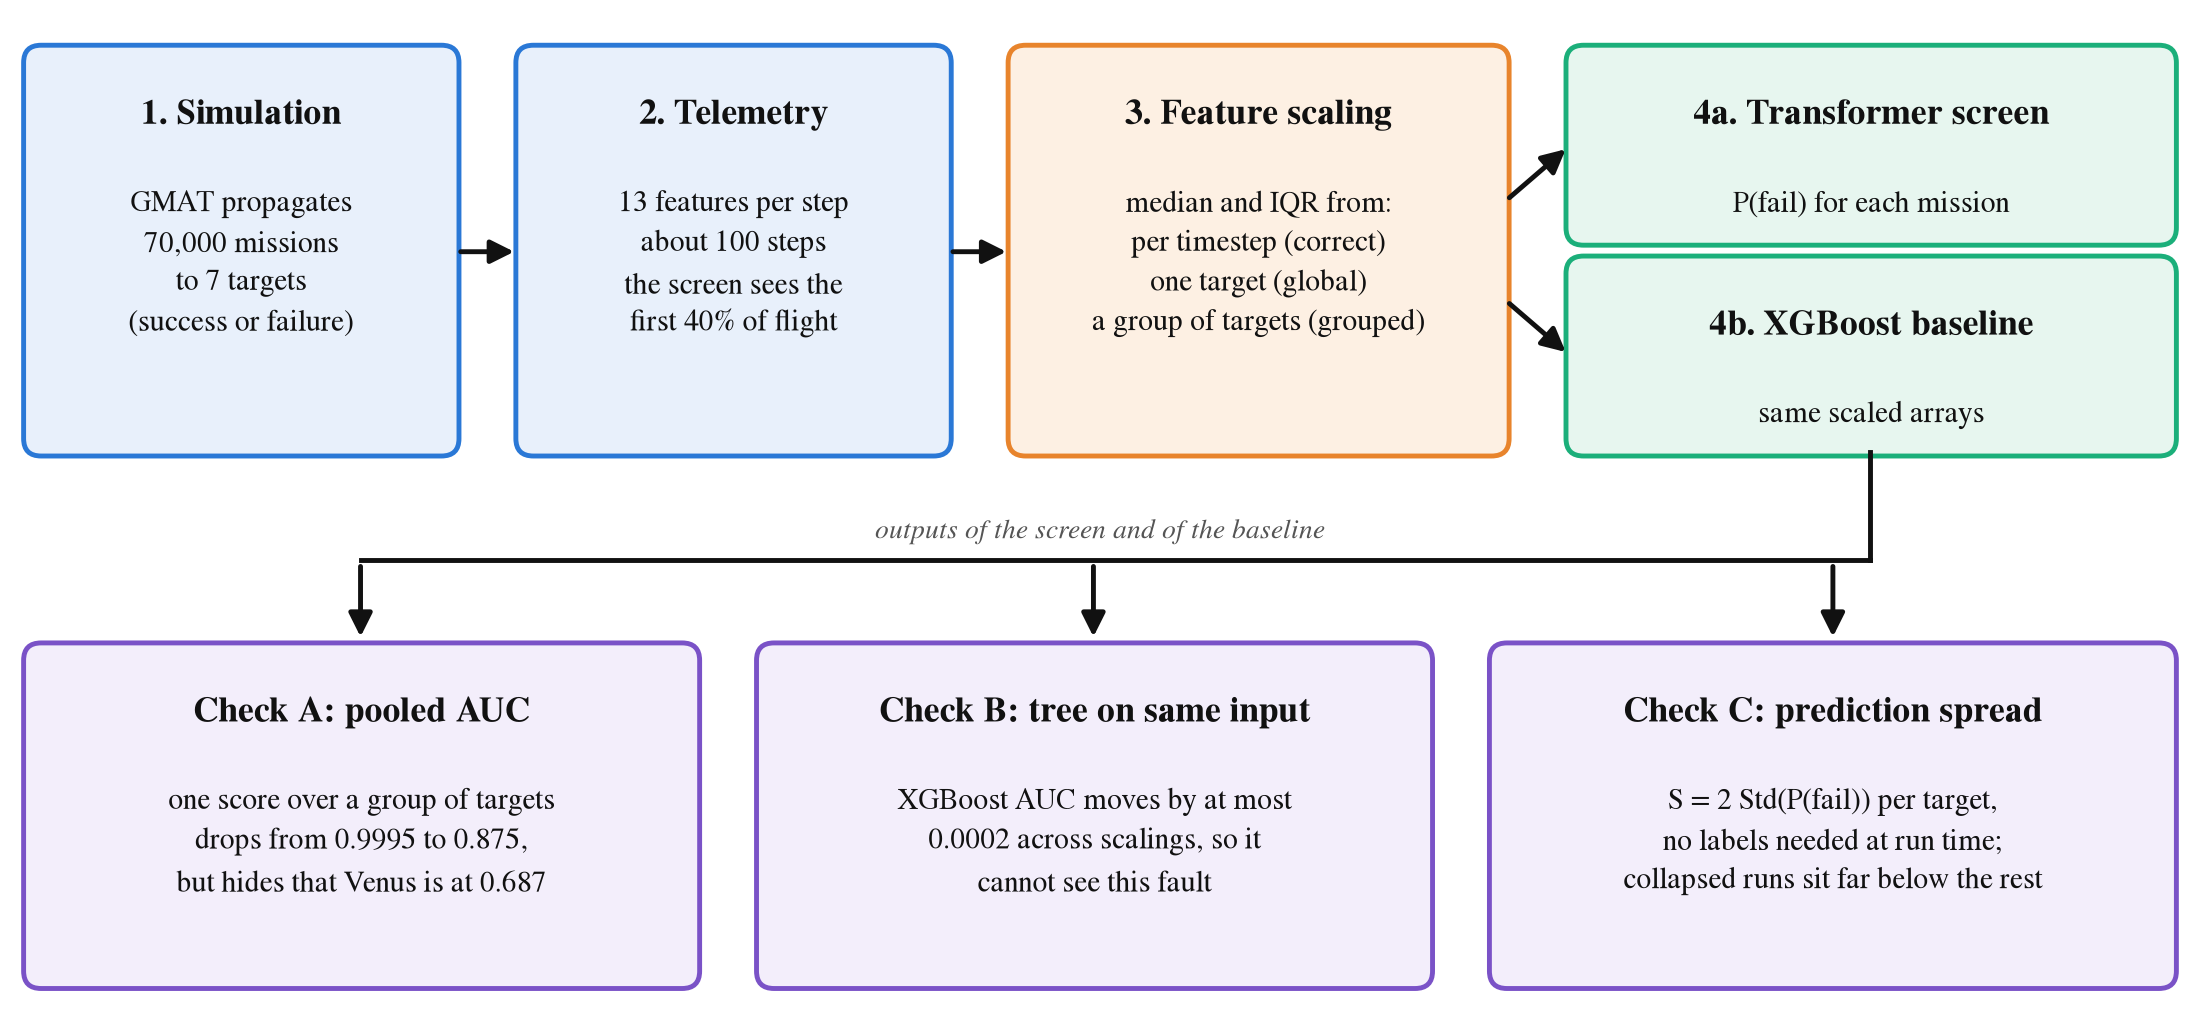
\includegraphics[width=\linewidth]{fig_pipeline.png}
\caption{Overview of the study. Missions are simulated, the first 40\% of each flight is scaled in one of three ways and passed to a Transformer screen and to an XGBoost baseline on the same arrays. The three checks at the bottom are compared in Section 4.}
\label{fig:pipeline}
\end{figure}

\subsection{Simulated mission data}

The data were generated with NASA's General Mission Analysis Tool (GMAT), an open source program for designing and analyzing space missions. Its propagator, the part that integrates the equations of motion forward in time, has been extensively verified for two and three body problems \cite{hughes2014}, and it is deterministic: the same inputs always give the same trajectory.

We simulated 70,000 missions that leave the Earth, 10,000 to each of seven interplanetary targets: Mercury, Venus, Mars, Jupiter, Saturn, Uranus and Neptune. Each mission starts from a parking orbit around the Earth and then performs a burn that puts the spacecraft on its transfer. Each mission has six injection offsets, which are small random changes to the mission plan. Three are the components of the transfer burn along the velocity, normal and binormal directions (dv\_V, dv\_N and dv\_B). The other three describe the orientation of the parking orbit: the right ascension of the ascending node (RAAN), the argument of periapsis (AOP) and the inclination (INC). Each mission is labeled a success or a failure, and failures are further divided into surface impact, an orbit that is too high, a missed target and a few other types. Table~\ref{tab:dataset} gives the size of each target set.

%%GENTABLE dataset%%

The transfers are sampled every 54,000 s (15 hours) and then downsampled to about 100 steps per mission, so that sequences from targets whose flight times differ by two orders of magnitude become comparable. Thirteen features are recorded at each step. Ten describe the motion: the position in a rotating (synodic) frame, the specific orbital energy, the flight path angle, the distance to the target divided by the size of its sphere of influence, the radial velocity toward the target, the speed, the distance from the Earth and the eccentricity. Three are constant for a mission and describe the target: the ratio of its gravitational parameter to the Sun's, the ratio of its sphere of influence to the transfer distance, and the transfer distance in astronomical units. An eighth target, the Moon, was simulated and deliberately left out. It is a six day transfer near the Earth, sampled every 60 s, with neither a cost structure like that of Section~\ref{sec:screen} nor a heliocentric regime.

The missions of each target are split by mission into 70\% for training, 15\% for validation and 15\% for testing. The split is a fixed function of the number of missions and the seed, defined once in the code, so no model is ever scored on data that were used for model selection. This is not a theoretical concern. Two earlier analyses in this project shuffled the same number of missions with the same seed in separate code, and the same missions ended up in both test sets.

\subsection{The screening task}

The screen observes the first 40\% of a mission's flight and decides whether to stop it. The model outputs P(fail), the probability that the mission fails. A threshold on P(fail), chosen on the validation split, turns this probability into a decision. The value of the screen is the propagation time it saves on failed missions, and its cost is the good missions it stops by mistake.

\subsection{Feature scaling}

Every setting uses robust scaling. For a feature value $x$, the scaled value is
\begin{equation}
z = (x - m) / q,
\end{equation}
where $m$ is a median and $q$ is an interquartile range (the distance between the 25th and 75th percentiles), both estimated on training data only. Robust scaling is a common choice because the median and the interquartile range are not moved much by outliers. The three settings differ only in which part of the data $m$ and $q$ come from (Fig.~\ref{fig:modes}).

\begin{itemize}
\item Per timestep. For each feature and each timestep index, $m$ and $q$ are taken over the training missions of one target at that index. This is the setting used by the working system.
\item Global. One median and one interquartile range per feature and target, pooled over all the timesteps of that target.
\item Grouped. One median and one interquartile range per feature, pooled over all the timesteps of all the targets in a regime group. The inner group is Mercury, Venus and Mars, and the outer group is Jupiter, Saturn, Uranus and Neptune. This is the setting that failed in our production system.
\end{itemize}

The grouped setting is not an artificial construction. A single robust scaler fitted to a concatenated training set is what many standard preprocessing tutorials produce. It raises no warning, and the result looks like an ordinary normalized array. Everything else (the architecture, the seed, the split, the optimizer and the number of epochs) is the same in all three settings.

%%FIGURE eaai:fig:modes%%

To measure how much useful variation survives the scaling, we use the signal ratio. It is the average standard deviation of the scaled features across missions, computed at each timestep and averaged over the observed window only. The window matters. Averaged over the entire flight the measure is uninformative: late timesteps have a large spread across missions, because the missions that fail have physically diverged by then, and this spread swamps the early signal, so all settings appear alike. The model commits at 40\% of the flight, so the relevant range is the one inside the prefix that the model observes.

\subsection{Models}

The screen is a Transformer encoder. A Transformer reads the whole sequence at once and uses attention to let every timestep look at every other one, which makes it a strong and widely used model for sequences. Our encoder uses pre-layer normalization (Pre-LN), a model width of 128, 8 attention heads and 4 layers. A learned summary token (CLS) is added to the start of the sequence, and its output is used to make the prediction. Two output heads share this trunk: one predicts whether the mission fails and one predicts the type of failure. The model is trained on prefixes of random length, so that it can give a prediction at any point in the stream and not only at the 40\% mark.

The baseline is XGBoost, a gradient boosted ensemble of decision trees, with 300 trees of depth 5. It is fitted to the same scaled prefix, flattened into one row per mission. It is important that the baseline does not work from a separately designed feature set but from the same view that the network sees. This is what the same input means throughout this paper, and it carries most of the argument. Table~\ref{tab:hyper} lists the training settings.

%%GENTABLE hyper%%

\subsection{The prediction spread diagnostic}
\label{sec:diag-method}

A collapsed model gives nearly the same P(fail) to every mission, so we look at how much its predictions vary. For a group $g$ with a batch of predictions $\hat{p}_i$, the group spread is the standard deviation of those predictions, $s_g = \mathrm{sd}(\hat{p}_i)$. The score we report is
\begin{equation}
S = 2 s_g,
\end{equation}
which runs from 0 for a constant output to 1 for the widest spread a probability can have (half of the predictions at 0 and half at 1). It needs no labels at inference time and no second model. Labels are used only during development, to say which runs have collapsed and to set the threshold. A second score divides by the spread of a healthy model trained on the same data:
\begin{equation}
D = s_g / (s_{\mathrm{healthy}} + \epsilon).
\end{equation}
It needs a model that was trained the right way, and when something is broken that is exactly what we do not have. We therefore use $S$ as the main score and report $D$ for comparison. We also compare $S$ with three other label-free summaries of the same predictions: the interquartile range, the range, and the mean binary entropy.

To have models in every state, we repeat the ablation on 5 seeds, 4 targets (Venus, Mars, Mercury and Jupiter) and the 3 scaling settings, which gives 60 runs, and keep the predictions on the validation and test missions of each run. The settings give four states. Per timestep runs are healthy, global runs are mildly hurt, grouped runs that keep working are severely hurt, and grouped runs that cannot rank missions are collapsed. A run counts as collapsed if its AUC on the split in question is 0.85 or lower.

The choices in this evaluation were made in the following order, and we state them plainly because the order matters. The group definitions and the three scaling settings come from the ablation. The AUC cutoff of 0.85 was set after the validation and test AUCs of all 60 runs had been seen. It was placed in the largest gap of the test AUCs (0.82 to 0.895) and of the validation AUCs (0.81 to 0.907), so it was not chosen in advance, and test results influenced it. Given the cutoff, the spread threshold was chosen on validation predictions and validation AUCs only: it is the middle, on a log scale, of the gap between the largest $S$ of a collapsed run and the smallest $S$ of a working run. The test predictions were used afterwards, to count the flagged runs. Because of this order, the test result is a check of the threshold and not an independent test of the cutoff, and Section~\ref{sec:check} reports how the result changes with the cutoff and when the threshold is set on other seeds.

\subsection{Evaluation metrics}

The main measure of ranking quality is the area under the receiver operating characteristic curve (AUC). It is the probability that a randomly chosen failed mission receives a higher P(fail) than a randomly chosen successful one, so 0.5 is chance and 1.0 is a perfect ranking. Because AUC depends only on the order of the predictions, it cannot tell a weak model from a constant one on its own, which is why we also report the spread of the predictions. For the screening decision we report the failure recall (the share of failed missions that are stopped), the share of good missions lost (successful missions that are stopped by mistake) and the F1 score of the failure class. The economic measure is the share of propagation time saved, where each mission is charged its propagation time, so outer planet missions weigh much more than inner ones.

\subsection{Statistical analysis}

Five seeds are few, so we report the individual runs rather than fitted intervals wherever possible. For the comparison of per timestep and grouped scaling on the same test missions we use three tests, computed from the saved predictions without retraining. First, a paired bootstrap with 2,000 resamples of the test missions gives a 95\% interval for each AUC and for their difference. Second, McNemar's exact test on the decisions at P(fail) of 0.5 asks whether the grouped model gets a different set of missions wrong. Third, Welch's t-test compares the test AUCs of the two settings across the five seeds. For the share of seeds on which the collapse occurs we give a 95\% Wilson interval.

\subsection{Second dataset}

To see what happens outside our simulator we used the NASA C-MAPSS turbofan data \cite{saxena2008}, a standard public set for remaining useful life work \cite{li2018rul}. It contains run to failure sensor records for fleets of aircraft engines. Subset FD001 has one operating condition, and FD002 and FD004 have six. The six conditions play the role that the targets play in our data: the sensors sit at very different levels in each one, and the slow drift that shows an engine wearing out is small next to that gap.

The task is to look at the last 30 cycles of an engine and say whether it will fail within the next 30 cycles. The split is by engine, 70/15/15, so no engine is in two sets. We scale the 14 sensors that change over an engine's life in two ways: pooled, with one median and interquartile range for every row, and per group, with one for each operating condition. The model is the Transformer described above with the same optimizer, trained for 20 epochs on 5 seeds, and the baseline is XGBoost on the same scaled window. FD001 has a single condition, so the two scalings are the same there, and it serves as the control.

\subsection{Implementation details and use of AI tools}

All experiments were run with PyTorch 2.13 and XGBoost 3.4.1 on one NVIDIA GeForce RTX 4060 laptop GPU with 8 GB of memory. One run of the ablation takes about 90 s to 3 min. Every number in this paper is read from machine-readable result files written by the experiment scripts, and the tables and figures are generated from those files.

During the preparation of this work the authors used Claude (Anthropic) to write and debug the experiment code, to draft the text of all sections, and to check the references and the numbers against the result files. The authors reviewed, edited and verified the content and take full responsibility for it.

\section{Experimentation and results}
\label{sec:results}

\subsection{Normalization ablation}

The first result is a controlled decomposition (Table~\ref{tab:ablation}). Pooling across time within a single target (the global setting) reduces the signal by up to a factor of 23, and the network still works on all four targets, with a loss of a few thousandths of AUC at most. In contrast, pooling feature statistics across heterogeneous target groups produces substantially more severe degradation, including near-constant predictions for Venus: the output standard deviation is 3.11e-05, which is one value for every mission, and the validation AUC drops from 0.9999 to 0.6037.

%%TABLE eaai:tab:ablation%%

We use the term collapse and not underfitting because of Fig.~\ref{fig:venus}. A low AUC alone is ambiguous, since it is also produced by a model that has learned something poor or wrong. A predicted distribution on unseen missions that is three ten-thousandths wide is not ambiguous: the output no longer depends on the input.

%%FIGURE eaai:fig:venus%%

The collapse is selective, and we report it together with the cases that do not break. On the remaining three targets the same manipulation leaves the output varying and costs between 0.0003 and 0.0925 AUC. The signal ratio is not a measure of severity either. Jupiter compresses its signal to 0.0247 and Mercury to 0.0484, yet Jupiter loses 0.0003 AUC while Mercury loses 0.0925. One explanation is that the Jupiter task is easily separable, so that even a very weak signal is sufficient. We did not test this directly. Compression is necessary for the collapse but not sufficient, and how hard the underlying task is appears to modulate it. We do not claim that these data support a rule of the form "it collapses when the ratio is below a given value". The counterexample is visible in Fig.~\ref{fig:signal}.

%%FIGURE eaai:fig:signal%%

This ablation isolates normalization and no other part of the model: only the statistics are pooled, and one model is trained for each target. The production failure also shared a single trunk across the group, which makes things worse, since one trunk then has to serve targets whose inputs have all been flattened toward a constant. These numbers are therefore a lower bound on the damage of that configuration. They show that pooled normalization is enough on its own to destroy a target, not that this is a complete reconstruction of the original incident.

\subsection{The tree baseline on the same input}

Under the grouped setting the XGBoost baseline reports an AUC of 1.0000 on Venus, the target where the network has collapsed to a constant at 0.6037 (Table~\ref{tab:xgb} and Fig.~\ref{fig:tree}). Its AUC changes by at most 0.0002 across the three settings on all targets, so this scaling choice is not visible to this baseline. The baseline therefore shows that the transformed arrays still contain an ordering that separates the classes. It does not show that the deep model can use the remaining small variation.

%%TABLE eaai:tab:xgb%%

%%FIGURE eaai:fig:tree%%

The exact claim matters here. The information is present, and this tree can use it. The comparison does not answer the question that has to be answered, which is whether the network can use the compressed signal. Its invariance to this rescaling makes the check blind to this particular defect. That statement is deliberately narrower than a claim that tree baselines cannot find preprocessing errors in general.

\subsection{Stability across random seeds}

A single run could be unlucky, so we repeated the whole ablation with five seeds. Each seed redraws both the train, validation and test partition and the initialization of the network. The compression does not depend on the seed. The signal ratio for Venus under grouped scaling lies between 0.00222 and 0.00232 across all five runs, a spread of 5\% against a compression of 335 times. The healthy setting is stable as well: the per timestep AUC of two different seeds differs by at most 0.0010, and Mars, Mercury and Jupiter do not collapse on any seed (Table~\ref{tab:multiseed} and Fig.~\ref{fig:seeds}).

%%TABLE eaai:tab:multiseed%%

%%FIGURE eaai:fig:seeds%%

Whether the network escapes does depend on the seed. Venus falls below a spread of 10\textsuperscript{-3} on 4 of 5 seeds, with a prediction spread on unseen missions between 1.57e-05 and 4.84e-05, four orders of magnitude below the 4.66e-01 of correct normalization. On the remaining seed it does not collapse, and it does not recover either: its prediction spread of 3.64e-02 is still an order of magnitude short, at an AUC of 0.9305 against a healthy 0.9999. The observed recurrence of 4 out of 5 has a 95\% Wilson interval of 0.376 to 0.964. That wide interval describes how often the collapse recurs under these seeds. It is not an interval for the sensitivity of a detector, and it does not support universal reliability.

This seed-to-seed variation is the main reason for the spread diagnostic. The grouped AUC of Venus ranges from 0.5338 to 0.9305 across these runs, which overlaps the AUC of a merely weakened target: Mercury lies inside that range on every seed while still telling missions apart. AUC alone therefore cannot separate the two states, while the prediction spread can. The invariance of the baseline is also repeated. Across 5 seeds, 4 targets and 3 settings, which is 60 fitted XGBoost models, the AUC stays between 0.9989 and 1.0000, and within each seed and target it changes by at most 0.0003 between settings.

\subsection{Statistical significance}

Table~\ref{tab:signif} compares per timestep and grouped scaling on the same test missions. On seed 42 the bootstrap interval of the AUC difference excludes zero for Venus, Mars and Mercury, and McNemar's test shows that the grouped model gets a different set of missions wrong on those three targets. For Venus, the grouped model is wrong on 974 test missions that the per timestep model gets right, against 9 the other way. For Jupiter the difference is small, and its interval touches zero. Over all 20 pairs of target and seed, the bootstrap interval of the AUC difference excludes zero in 16 and McNemar's test is significant in 16. The two tests agree on 15 pairs, and the two pairs where they disagree are both Jupiter runs. Across the five seeds, Welch's t-test separates the two settings for Mars, Mercury and Venus, and not for Jupiter. These tests confirm that the damage is real and not a chance result of one split. With five runs per setting, however, they say nothing about how often such a collapse would occur in other pipelines.

%%GENTABLE signif%%

\subsection{Evaluating the prediction spread check}
\label{sec:check}

The four collapsed runs are exactly the four that fall below the earlier, stricter rule of a group spread under 10\textsuperscript{-3}. At the AUC cutoff of 0.85, the spread threshold chosen on validation is 2.7e-03, in the middle of the gap between the largest $S$ of a collapsed run (1.0e-04) and the smallest $S$ of a working run (0.071). Applied unchanged to the test predictions, it flags 4 runs out of 60, which are the 4 with a test AUC of 0.85 or lower, and no working run (Table~\ref{tab:states} and Fig.~\ref{fig:check}). The score $D$, with its threshold chosen the same way, flags the same 4, so the reference model did not add anything here.

%%TABLE eaai:tab:states%%

%%FIGURE eaai:fig:check%%

The score is meant for collapse, not for every loss of accuracy. The Mercury runs under grouped scaling lose about 0.09 AUC while their spread stays above 0.76, so the check does not flag them. Venus on seed 3 is the hard case. Its $S$ is 0.073, about ten times below a healthy run, and it still ranks missions at an AUC of 0.92. It is above the threshold and is not flagged.

Table~\ref{tab:cutoffs} shows how the result depends on the AUC cutoff. A single threshold can be set on the validation runs only at cutoffs of 0.85 and 0.90. Below 0.85 the Venus run on seed 2, with a validation AUC of 0.81, is labeled as working, but its spread (7.9e-05) lies inside the range of the collapsed runs, so no threshold separates the two labeled groups. At 0.95 fourteen runs count as collapsed, including Mercury runs that keep their spread, and the groups overlap again. The ranking is more stable than the threshold: the ROC AUC of $S$ on the test predictions is 1.000 for every cutoff from 0.60 to 0.85 and 0.993 at 0.90. The score separates runs with a near-constant output from the others. Whether a run with a constant output but a usable ranking, such as Venus on seed 2, is called collapsed depends on the cutoff.

%%TABLE eaai:tab:cutoffs%%

To test the threshold on seeds it was not chosen on, we set it on the validation predictions of four seeds and applied it to the test predictions of the fifth, for each seed in turn. At a cutoff of 0.85 this gives 4 collapsed runs, 0 missed and 0 false alarms over the 60 runs. At 0.90 there are 5 collapsed runs, 1 missed (a Mercury run that keeps its spread) and 0 false alarms. At the lower cutoffs no threshold could be set on some of the seeds, for the reason given above. These seeds redraw the split and the initialization, but they use the same four targets, so this is not a test on new targets.

The statistic is an ordinary output variance, and we do not claim that it is the best summary. Table~\ref{tab:cutoffs} also gives the ROC AUC of three other label-free summaries of the same predictions. Up to a cutoff of 0.85 all of them separate the collapsed runs well (0.98 to 1.00). At 0.90 the spread score is the highest (0.993, against 0.989 for the entropy, 0.978 for the range and 0.945 for the interquartile range), and at 0.95 the range and the entropy are higher than it. The differences are small and rest on four collapsed runs from one target. What these results support is that a summary of the predictions computed per group detects a failure that the tested baseline does not detect and that a pooled score shows only in part. They do not support a claim that this score is better than other output summaries.

A pooled score shows the collapse only in part. For the inner group (Mercury, Venus and Mars) the AUC over the test missions of all three targets is 0.9995 with per timestep scaling and 0.875 with grouped scaling, averaged over the five seeds. That is a visible drop. It is, however, 0.19 above the AUC of Venus alone (0.687) and above the mean of the three per target AUCs (0.845), because a model that is constant within a group still ranks the groups against each other. The pooled value also does not say which target failed. The spread is computed per target, and it is 3.1e-05 to 9.7e-05 for the four collapsed Venus runs, against 0.7 or more for Mercury and Mars under grouped scaling.

The spread is computed over a batch of predictions, so it depends on the batch size and on how the probabilities are calibrated. We resampled the saved test predictions at random. Batches of 30 or more missions flagged every collapsed run and no working run. Batches of 10 flagged 1.1\% of the working batches, and batches of 5 flagged 7.4\%. These batches contain both outcomes, because they were drawn at random from the test missions. A batch that holds missions of one outcome only, or from one narrow region of the inputs, was not tested, and a small spread would be expected there. We also rescaled the predicted log-odds by a temperature between 0.25 and 4. The smallest spread of a working run then moved between 0.28 and 0.018, and the threshold of 2.7e-03 still separated the 4 collapsed runs from the 56 working runs. This is a monotone change of the outputs of one model family. A model with different calibration, architecture, label prevalence or batch size needs its own threshold.

The signal ratio can be measured before any training, so it can serve as an early warning. Every collapsed run has a signal ratio of 0.0022 or 0.0023. Five runs are below 0.01, namely the 4 collapsed runs and Venus on seed 3, and no run at 0.0243 or above collapsed. The ratio can therefore warn that a configuration is at risk, but it cannot say which of the runs will collapse. For that, the spread after training is needed.

\subsection{Second dataset}
\label{sec:second}

On the turbofan data, pooling shrinks the signal about nine times, from 0.802 to 0.083 on FD002 and from 0.859 to 0.097 on FD004. The model does not break (Table~\ref{tab:cmapss}). On both subsets the pooled Transformer is slightly ahead of the per group one, the spread of its predictions is the same, and the tree performs well either way. The spread check, with the threshold it already had, flags none of the 30 runs.

%%TABLE eaai:tab:cmapss%%

This agrees with the ablation. Shrinking the signal is not enough to break a model: in our data Mercury and Jupiter lose most of their signal under grouped scaling and keep working, and here the drift is still present after pooling and the model finds it. It also shows that the check does not raise an alarm on a second kind of data. It does not show that the threshold carries over to other domains.

\subsection{Where the screen belongs}
\label{sec:screen}

The final question is whether a sequence model is the right tool for this screen at all. A classifier that uses only the six injection offsets, and is applied before any propagation, saves 64.5\% of the compute, against 38.3\% for the telemetry Transformer at 40\% of the flight, at a similar cost in good missions lost (Table~\ref{tab:economics}). Accuracy also levels off between 10\% and 40\% of the flight. This is not a modeling fault. The simulator is deterministic, so the outcome is a fixed function of the injection offsets, and the trajectory is an integral of those offsets. It cannot carry information that the offsets do not have.

%%TABLE eaai:tab:economics%%

This does not make the task trivial. Logistic regression on the same six offsets reaches only 0.4824 to 0.5410 AUC on the seven targets, which is chance, so the mapping from the offsets to the outcome is highly nonlinear and needs a learned model. It does not need a temporal one. A sequential screen is worth using only when the outcome is not fixed at injection: with stochastic effects during flight, unmodeled dynamics, sensor noise, or campaigns where the launch parameters are unknown. That is the setting that reinforcement learning trajectory work faces when it certifies policies through dispersed Monte Carlo campaigns \cite{zavoli2021}. For the T0 screen, a five-split analysis (seeds 0 to 4) gives compute saved of 64.50\% $\pm$ 0.61 percentage points, good missions lost of 1.24\% $\pm$ 0.24, and failure recall of 98.99\% $\pm$ 0.18 (mean and standard deviation across five splits). The T40 and cascade rows remain single seed estimates. Five correlated resplits of one synthetic corpus do not measure uncertainty across campaigns or domains.

\section{Discussion}
\label{sec:discussion}

\subsection{What the results mean for mission assurance}

The first paragraph below states what the experiments in this paper show. The second and third describe consequences and a workflow that have not been tested.

\textbf{Demonstrated result.} Within the GMAT experiment, the per target spread of the predictions exposes four near-constant Venus runs that the tested XGBoost comparison does not identify and that a pooled AUC shows only in part. Because it checks the behavior at the interface between preprocessing and model, the same kind of check can support verification and validation in other simulation screening pipelines: it tests whether changing the candidate inputs still changes the output of the learned screen. It does not validate the trajectory propagator, prove physical correctness, certify flight software, or establish a threshold outside the evaluated configuration.

\textbf{Operational implication.} If a similar collapse went unnoticed in a mission design campaign, the screen could assign nearly the same decision to very different candidates. Depending on that constant and on the decision threshold, it could discard viable trajectories, keep expensive failures, distort estimates of the size of the feasible region, and bias trade studies or robustness margins. A healthy score from other target groups could hide the affected group and create false confidence in the campaign. These consequences are analyses of possible failures, not outcomes measured in a flight campaign.

\textbf{Proposed pipeline.} During development, a team would generate labeled working, degraded and deliberately broken validation states for each combination of dataset, architecture, target group and preprocessing version. It would set a group-specific spread threshold and a minimum batch size on those states, freeze both before the untouched test evaluation, and record false alarm and miss rates with their uncertainty. At run time, each screening batch would log the versions of the model, scaler, data and groups, compute the group spread alongside input-signal and feature-shift checks, and compare only with the matching frozen limits. An alarm would set the learned screen aside, keep all candidates, and fall back to full propagation rather than stopping trajectories. A tree comparison can help offline diagnosis by asking whether information remains in the same arrays, but it is not needed to compute the run-time statistic.

\subsection{Limitations}

\begin{itemize}
\item Seeds. Replication is limited to 5 seeds. The observed recurrence of 4 out of 5 has a wide 95\% Wilson interval (0.376 to 0.964), and five seeds rule out neither an unknown controlling factor nor substantial uncertainty.
\item Threshold. The AUC cutoff that defines a collapsed run (0.85) was set after the validation and test AUCs had been seen. The spread threshold (2.7e-03) was chosen on validation predictions only, so the test result is a check of that threshold and not an independent test of the cutoff. A single threshold can be set only for cutoffs of 0.85 and 0.90. All 4 collapsed runs are Venus, so one kind of collapse has been tested. The threshold is not expected to transfer unchanged to another dataset, architecture, calibration, target group, prevalence or batch size, and batches with one outcome class were not tested.
\item Datasets. The collapse is shown on the GMAT corpus. The turbofan data show the same loss of signal without a collapse and without an alarm. That supports the absence of false alarms there, but it does not show that the threshold carries over to other domains.
\item Targets. One of four targets collapses, and all collapsed runs are Venus. Other target combinations and group definitions are needed to estimate how much the composition of a group matters.
\item Architecture. An LSTM control on the ordinary, correctly preprocessed screening task reaches a test AUC of 0.9928 against 0.9958 for the Transformer, so the base task is not unique to one architecture. The LSTM was not run under grouped scaling, so whether the collapse occurs beyond the Transformer remains open.
\item Severity. The check flags near-constant output. It does not flag a model that loses accuracy but keeps its spread, such as Mercury, and graded compression sweeps were not built.
\item Synthetic and deterministic data. There are no execution errors, no unmodeled accelerations and no sensor noise, and all missions of a target share a common time base. That common time base is what makes per timestep scaling possible, and it is a property of the generator rather than of a real campaign. Public satellite telemetry benchmarks \cite{kotowski2024,hundman2018} are a natural next place to test the check.
\end{itemize}

\section{Conclusion and future work}
\label{sec:conclusion}

When one scaler is pooled across groups with different scales, the tested Transformer can turn into a constant for one group, while the tested scale-invariant XGBoost baseline still finds the same arrays separable and a pooled validation score shows the damage only in part. None of the pieces here are unusual. The defect enters through a routine preprocessing step, the model is a plain Transformer, and the baseline is the one most practitioners would choose. The conclusion is not that trees cannot diagnose preprocessing errors, but that a check which is invariant to this transformation cannot answer whether a scale-sensitive network can use the compressed signal.

We do not claim that the fix, normalizing each group separately, is new. The lesson is about detection: monitor the behavior of the outputs within each group, in addition to pooled scores and baselines. Computing the prediction spread needs no labels at run time, but turning it into an alarm needs a threshold set for each model version and an independent labeled evaluation during development. On a second dataset, where pooling shrank the signal and the model survived, the same check raised no alarm.

Future work should test the check on real telemetry, on other architectures such as LSTMs trained under grouped scaling, on more target groups and group definitions, and on graded levels of signal compression, with the threshold fixed before any test data are seen. For trajectory screening in particular, a screen based on the injection parameters should be preferred whenever the simulator is deterministic, and a sequential screen should be reserved for campaigns in which the outcome is not fixed at injection.

\section*{Data availability}

The simulated mission data were generated with NASA's General Mission Analysis Tool. The per target extracts used in the experiments can be regenerated with the scripts in the code repository and are available from the corresponding author on reasonable request. The full mission table (about 71 GB) is too large to share in a public repository. The NASA C-MAPSS turbofan engine degradation data are publicly available from the NASA Prognostics Center of Excellence data set repository.

\section*{Code availability}

The code for all experiments, the result files from which every number is read, and the code that produces the tables and figures are available at https://github.com/Haise-727/gmat-pred.

\section*{Funding}

The authors received no funding for this work.

\section*{Author contributions}

Harsha Vardan M Sakamuri: conceptualization, methodology, software, validation, formal analysis, investigation, data curation, writing of the original draft, review and editing, visualization. Rohit Michael Raj: conceptualization, methodology, software, validation, formal analysis, investigation, data curation, writing of the original draft, review and editing, visualization. Valarmathi P.: supervision.

\section*{Competing interests}

The authors declare no competing interests.
